\subsection{Registracion y Ingreso al casino online y modificacion de saldo}

\subsubsection{Registracion}
Segun lo acordado, la registracion de los usuarios de hace por fuera del sistema informatico del casino online. Explicaremos como esperamos que interactuen los agentes externos para que el sistema posea la lista actualizada de usuarios registrados. Para ello usaremos el Diagrama de Activdades\footnote{Diagrama de Actividades: Grafico que representa el flujo de actividades. Las cajas representan actividades y las flechas repersentan secuencialidad y los rombos representan decisiones} ``Registracion''. Ver Figura: \ref{fig:daReg}

\begin{figure}[h!]
	\centering
		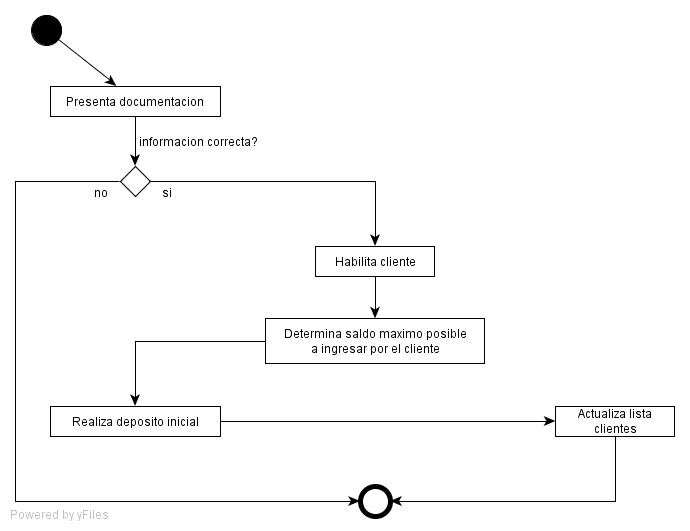
\includegraphics[scale=0.5]{img/daRegistracion.png}
	\caption{Diagrama de actividades Registracion\label{fig:daReg}}
\end{figure}

Cabe aclarar que el cliente podra comenzar a jugar en el casino recien cuando el casino se vuelva a abrir

\subsubsection{Modificacion de saldo}

Una vez registrado un cliente puede ingresar y retirar dinero real, dicha operacion solo podra realizarse mistras el casino permanece cerrado.
Explicaremos esta operatoria con un diagrama de actividades. Ver Figura: \ref{fig:modSaldo}

\begin{figure}[h!]
	\centering
		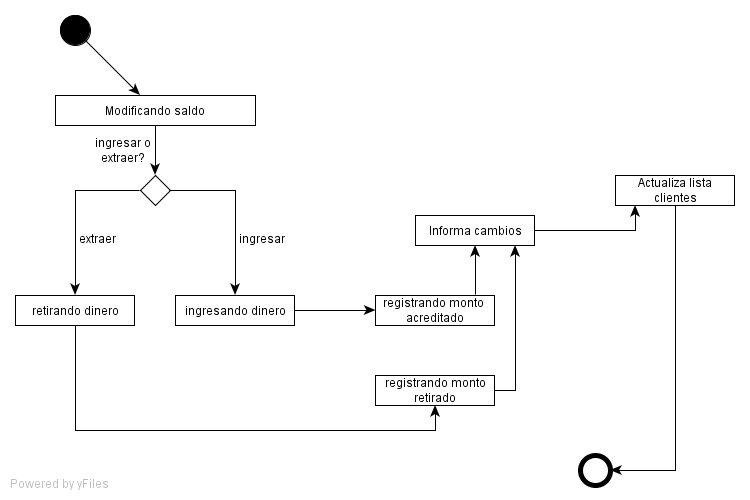
\includegraphics[scale=0.5]{img/clienteModSaldo.png}
	\caption{Diagrama de actividades Modificacion de Saldo\label{fig:modSaldo}}
\end{figure}

\subsubsection{Ingreso y egreso del casino}

La forma en que un cliente ingresa o egresa del casino esta explicado en los casos de uso: \\
CU \ic \ref{lic} y CU \salc \ref{lsalc}.

\subsection{Administracion del Casino}

\subsubsection{Apertura del casino}

En el momento de la apertura del casino es podible realizar configuraciones distintos aspectos:
\begin{itemize}
	\item Configuracion de valores de fichas
	\item Asignacion de probablilidades
	\item valores minimos para la entrega de premios
\end{itemize}

Dicha interaccion con el sistema esta explicada en el caso de uso: CU \ac \ref{lac}

\subsubsection{Clausura del casino}

La operatioria de cerrar el casino no es muy complicada, pero tiene una salvedad. No es posible cerrar el casino si hay jugadores dentro del casino

Dicha interaccion con el sistema esta explicada en el caso de uso: CU \ccas \ref{lccas}

\begin{framed}

\depto Con esta maquina de estados finitos (FSM) Mostramos que nos comprometemos a que un administrador podr� cerrar el casino solo si no hay ningun cliente en el mismo.


{\large FSM: Administrador}
\begin{center}
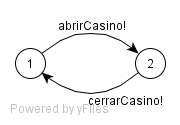
\includegraphics[scale=0.5]{img/admin.png}
\end{center}


{\large FSM: Jugador$_i$}
\begin{center}
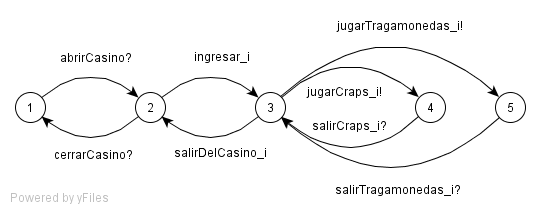
\includegraphics[scale=0.5]{img/jugador.png}
\end{center}

\textbf{Nota}: la interaccion que tiene un jugador con cada uno de los juegos se puede observar en los apartados `JUEGO TRAGAMONEDAS' y `JUEGO CRAPS'. 


\end{framed}

\subsection{Modo Dirigido}

\subsubsection{Inicio de Modo Dirigido}

Cuando se ingresa en este modo, los resultados de las jugadas no seran al azar sino que el manipulador decidira los mismos.

Esos resultados ingresados se respetaran para todas las jugadas de todas las mesas habilitadas de ese juego mientras no se vuelva a modo normal.

Dicha interaccion con el sistema esta explicada en el caso de uso: CU \actm \ref{lactm}
\begin{framed}

\depto Con esta maquina de estados finitos (FSM) Mostramos que en modo dirigido se pueden lanzar jugadas de forma manual, dicha funcionalidad no esta permitida en modo normal.
Es seteo de las jugadas debe hacerse en el momento de entrar en modo dirigido. 

\paragraph{FSM: Manipulador}
\begin{center}
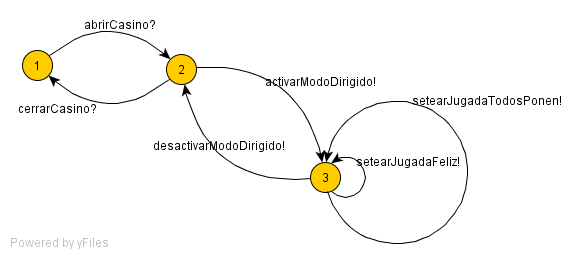
\includegraphics[scale=0.5]{img/manipulador.png}
\end{center}

\end{framed}

\subsubsection{Seteo de Jugadas Feliz y Todos Ponen}

El manipulador puede iniciar una Jugada Feliz, al hacerlo debe seleccionar una unica jugada que se ver� afectada por la Jugada Feliz.

Dicha interaccion con el sistema esta explicada en el caso de uso: CU \jugf \ref{ljugf}

Por otro lado, si el manipulador inicia una Jugada Todos Ponen, al hacerlo puede seleccionar varias jugadas las cuales se veran afectadas (todas) por la jugada de este tipo.

Dicha interaccion con el sistema esta explicada en el caso de uso: CU \jugtp \ref{ljugtp}

\subsubsection{Finalizaci�n de Modo Dirigido}

En el momento que el manipulador decida abandoanar el modo dirigido, debera desactivarlo.
Y asi volver al modo normal. Ver caso de uso: CU \desm \ref{ldesm}
                                            
\subsection{Juego Tragamonedas}

Las m�quinas tragamonedas juegan con un �nico valor de ficha (Cuando se inicia el jugador elige dicho valor, entre los valores de fichas disponibles del casino). 

En el siguiente Diagrama de actividades se puede observar a grandes rasgos las actividades que realiza un jugador de tragamonedas.

\begin{center}
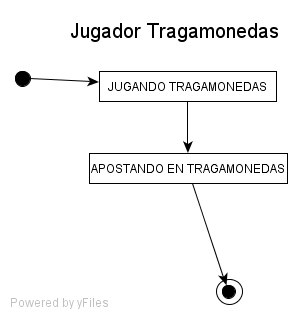
\includegraphics[scale=0.5]{img/JugadorTragamonedasDA.png}
\end{center}

Cada una de estas actividades se explican con mas detalle en los casos de uso: CU \jtra \ref{ljtra} y CU \apotra \ref{lapotra}

\begin{framed}

\depto Con esta maquina de estados finitos (FSM) mostramos el desarrollo del juego tragamonedas, modelando solo la parte de cobrar o no. 

{\large FSM: JugadaTragamonedas}
\begin{center}
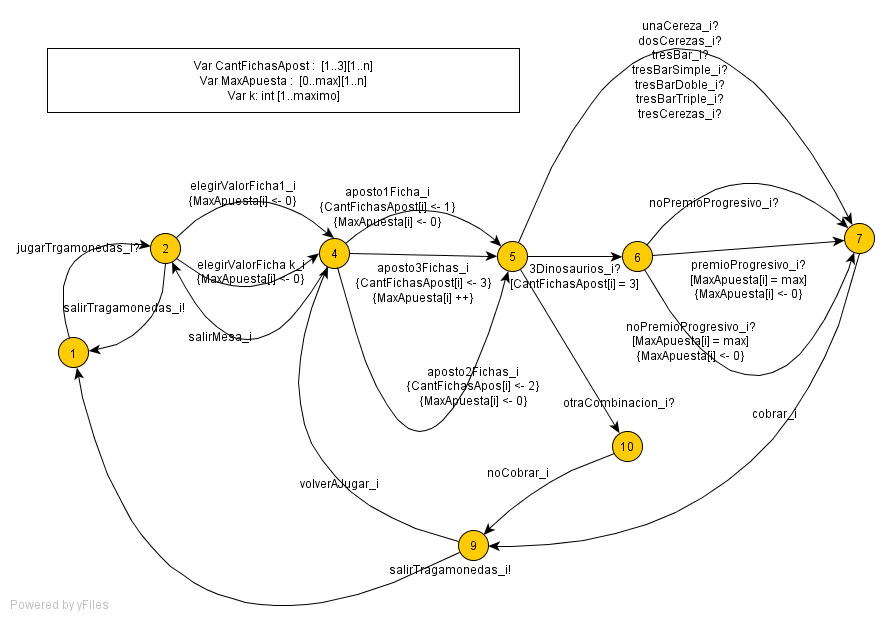
\includegraphics[scale=0.5]{img/JugadaTragamonedas.png}
\end{center}

{\large FSM: MaquinaTragamonedas}
\begin{center}
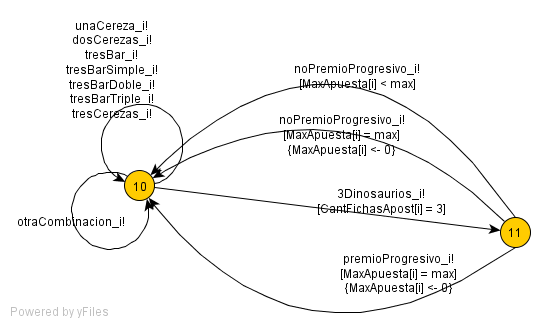
\includegraphics[scale=0.5]{img/MaquinaTragamonedas.png}
\end{center}

\textit{\textsl{Aclaraciones}}: 
\begin{itemize}
	\item{Dado que al abrir el casino se determina con que fichas se jugar�,\textit{\textbf{elegirValorFicha}} refiere a una de esas 	fichas. Es decir, que al abrir una mesa se debe elegir una ficha dentro de las posibles. }
	\item{Abuso de la notacion al referimos a los posibles resultado.}
	\item{Hay tantas FSM maquina tragamonedas como mesas se abran. Cuando
	el jugador sale de la mesa, esta queda inhabilitada para una proxima jugada}
	\item{De haber varias jugadas con posibilidad de ganar el premio progresivo, 	este ser� otorgado solo a una de ellas. 	En la FSM \textit{\textbf{JugadaTragamonedas}} se ve la flecha \textit{\textbf{nopremioProgresivo}} donde la apuesta es maxima, la cual refleja lo explicado previamente}
	\item{Si la apuesta es maxima la cantidad de apuestas de 3 fichas volver� a cero, tanto si gana el premio progresivo 	  o no lo gane}
\end{itemize}

\end{framed}

\subsection{Juego Craps}

Otro de los juegos elegidos por los socios es el \textbf{Craps}. En este juego un tirador lanza un par de dados para establecer un PUNTO y las apuestas girar�n en base a las posibilidades de que dicho tirador repita el mismo punto antes de lanzar un 7.
Cuando un jugador Craps decida jugar debe seleccionar una mesa existente o abrir una nueva. Luego durante el juego podra tirar los dados y/o apostar.

Cada una de estas actividades se explican con mas detalle en los casos de uso: \\
CU \incr \ref{lincr}, CU \jcr \ref{ljcr}, CU \apcr \ref{lapcr} y CU \scr \ref{lscr}

\begin{framed}

\depto Con estas maquinas de estados finitos (FSM) mostramos el desarrollo del juego craps. Incluyendo entre ellas un seleccionador, un tirador y cada una de las apuestas. 

{\large FSM: Seleccionador}
\begin{center}
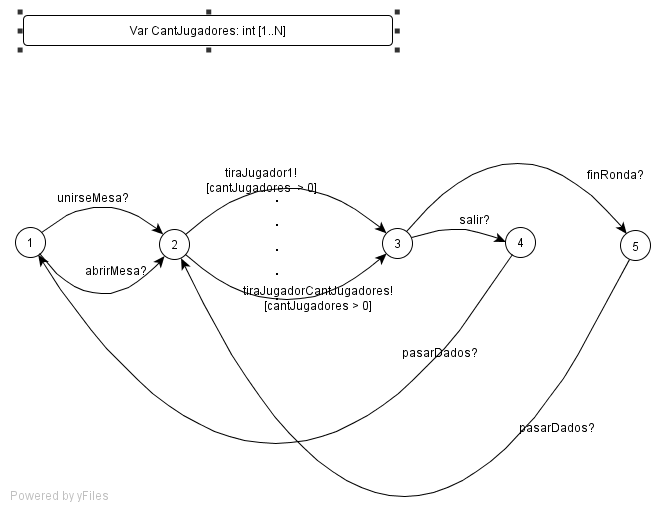
\includegraphics[scale=0.4]{img/seleccionador.png}
\end{center}

{\large FSM: Tirador}
\begin{center}
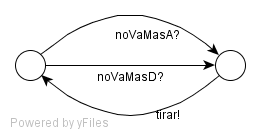
\includegraphics[scale=0.5]{img/tirador.png}
\end{center}

{\large FSM: Desarrollo Craps}
\begin{center}
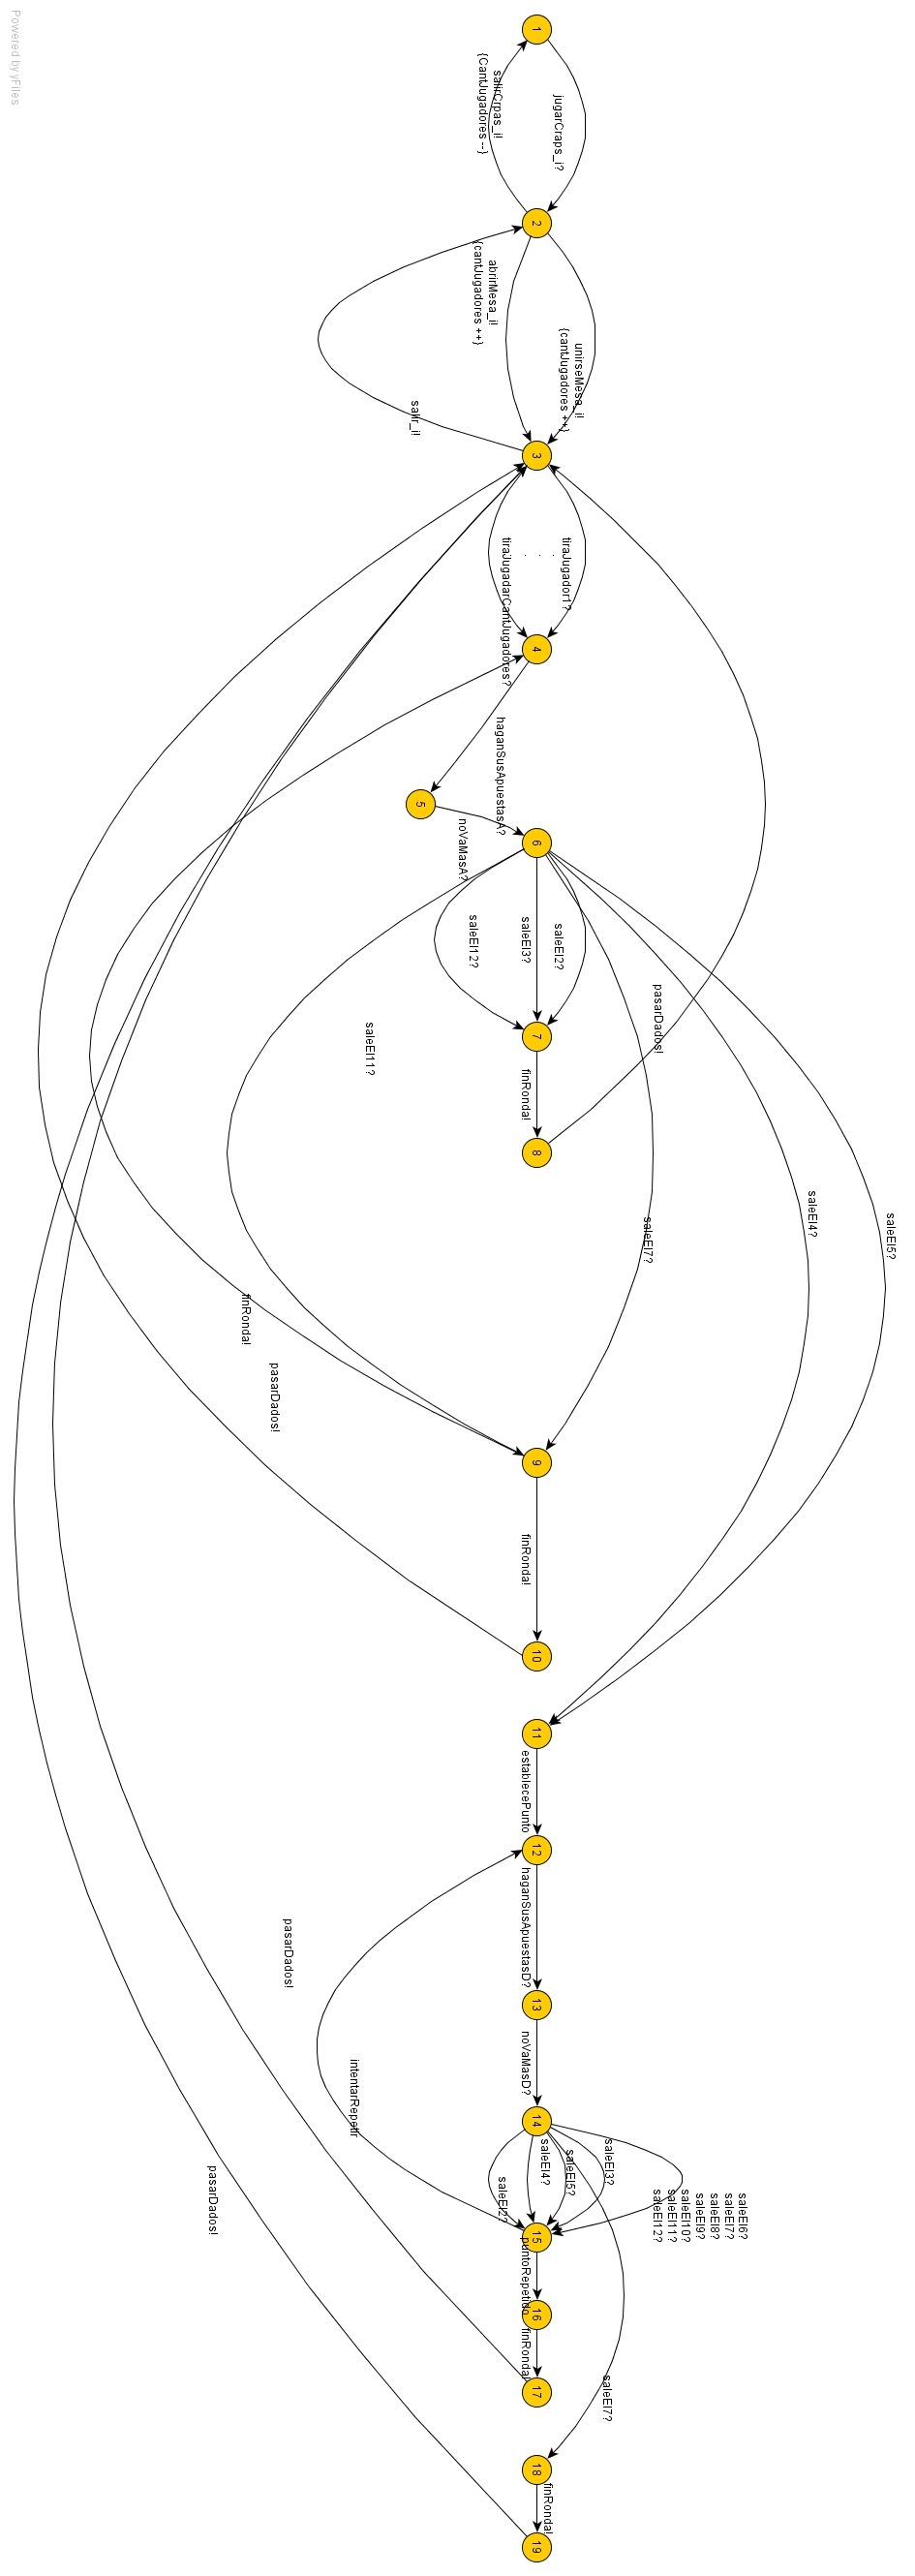
\includegraphics[scale=0.25]{img/desarrolloCraps.png}
\end{center}

\end{framed}

\subsection{Generacion de reportes}

Expicamos en lenguaje OCL como es que se obtienen los datos necesarios para la generacion de los informes.

\subsubsection{Generacion de reporte: Ranking de Jugadores}

\begin{framed}
\begin{lstlisting}[breaklines=true]
--este operacion devuelve dado un jugador una tupla con su nombre y su ganancia
dameNombreGanancia(j:Jugador):TupleType(nombre:String , ganancia: Numero))
pre:	true
post:	result = Tuple{nombre:String = j.nombre, ganancia:Numero = (j.saldo - j.saldoInicial)}


--genera el reporte de ganancia por jugador
--
--busco el jugador que mas gano
--y selecciono todos los jugadores que hayan ganado tanto como el que mas gano
--luego los transforno en tuplas
--
reporteRanking(ascendente:Boolean):Collection(TupleType(nombre:String , ganancia: Numero))
pre:	true
post:	
	let jugadores:Collection(Jugador) = Jugador.allInstances()
	let masGanadores = jugadores->orderedBy(j | j.saldo - j.saldoInicial)
	let menosGanadores = jugadores->orderedBy(j | j.saldoInicial - j.saldo)

if ascendente
then
	result = masGanadores->iterate(j;res=orderedSet();res->including(dameNombreGanancia(j))
else
	result = menosGanadores->iterate(j;res=orderedSet();res->including(dameNombreGanancia(j))
endif

\end{lstlisting}
\end{framed}

\subsubsection{Generacion de reporte: Estado Actual}

\begin{framed}
\begin{lstlisting}[breaklines=true]
--este operacion devuelve dado un jugador una tupla con su nombre y su saldo y el del casino
dameNombreSaldo(j:Jugador):TupleType(nombre:String , ganancia: Numero))
pre:	true
post:	result Tuple{nombre:String = j.nombre, saldo:Numero = j.saldo}

estadoActual(): Collection(TupleType(nombre:String , saldo: Numero))
pre:	true
post:	
	let jugadores:Collection(Jugador) = Jugador.allInstances() 
	let casino:Jornada = Jornada.allInstances()->asSecuence->first()

	result jugadores->iterate(j;res=orderedset();res->including(dameNombreGanancia(j))
		->including(Tuple{nombre:String = "Jornada Actual", saldo:Numero = casino.saldo})

\end{lstlisting}
\end{framed}

\subsubsection{Generacion de reporte: Detalle de movimientos por jugador}

\begin{framed}

\textbf{TINTERO: } No hemos podido llegar a terminar la operacion de ``Detalle de movimientos por jugador'', pero segun nuestro estudio nuestro modelo conceptual soporta la generacion de este reporte. 

\end{framed}

\subsection{Pago de jugadas y premios}

Se explicaran aqui con detalle como se refleja el pago de apuestas en el modelo propuesto (Modelo de Clases)\\

\textbf{NOTA: } Esta seccion esta dirigida a solo a lectores con conocimientos de modelo de clases conceptuales y OCL. 

\begin{itemize}
	\item Pago de una jugada tragamonedas. Ver Anexo \ref{an4}
	\item Pago de una jugada craps. Ver Anexo \ref{an5}
\end{itemize}
